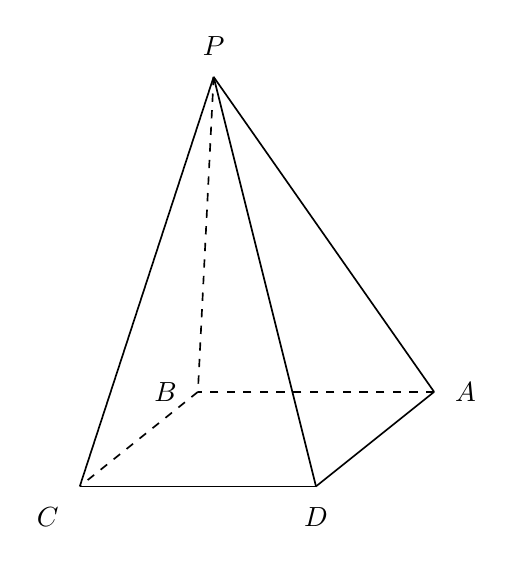
\begin{tikzpicture}[line width=.6pt, font=\normalsize]
\coordinate (B) at (1.5,1.2);
\coordinate (C) at (0,0);
\coordinate (D) at (3,0);
\coordinate (A) at (4.5,1.2);
\coordinate (P) at (1.7,5.2);
% base square ABCD (B back corner hidden)
\draw (C) -- (D);
\draw (D) -- (A);
\draw[dashed] (A) -- (B);
\draw[dashed] (B) -- (C);
% lateral edges, PB is the altitude (hidden)
\draw (P) -- (C);
\draw (P) -- (D);
\draw (P) -- (A);
\draw[dashed] (P) -- (B);
% labels with clearance
\node[above=4pt] at (P) {$P$};
\node[left=4pt] at (B) {$B$};
\node[below left=4pt] at (C) {$C$};
\node[below=4pt] at (D) {$D$};
\node[right=4pt] at (A) {$A$};
\end{tikzpicture}
